%% intro.tex
%%
%% Copyright 2017 Evandro Coan
%% Copyright 2012-2016 by abnTeX2 group at http://www.abntex.net.br/
%%
%% This work may be distributed and/or modified under the
%% conditions of the LaTeX Project Public License, either version 1.3
%% of this license or (at your option) any later version.
%% The latest version of this license is in
%%   http://www.latex-project.org/lppl.txt
%% and version 1.3 or later is part of all distributions of LaTeX
%% version 2005/12/01 or later.
%%
%% This work has the LPPL maintenance status `maintained'.
%% The Current Maintainer of this work is the Evandro Coan.
%%
%% The last Maintainer of this work was the abnTeX2 team, led
%% by Lauro César Araujo. Further information are available on
%% https://www.abntex.net.br/
%%
%% This work consists of a bunch of files. But originally there ware 3 files
%% which are renamed as follows:
%% Renamed the `abntex2-modelo-include-comandos` to `chapters/chapter_1.tex`
%% Renamed the `abntex2-modelo-trabalho-academico.tex` to `chapters/intro.tex`
%% Renamed the `abntex2-modelo-references.bib` to `aftertext/modelo-ufsc-references.bib`
%%
%% This file was originally the main template file, however this main file was
%% split into several new files, which are respectively drastically changed,
%% except this files which contains most of the main documentation message.
%%

% ------------------------------------------------------------------------
% ------------------------------------------------------------------------
% abnTeX2: Modelo de Trabalho Academico (tese de doutorado, dissertacao de
% mestrado e trabalhos monograficos em geral) em conformidade com
% ABNT NBR 14724:2011: Informacao e documentacao - Trabalhos academicos -
% Apresentacao
% ------------------------------------------------------------------------
% ------------------------------------------------------------------------


% The \phantomsection command is needed to create a link to a place in the document that is not a
% figure, equation, table, section, subsection, chapter, etc.
%
% When do I need to invoke \phantomsection?
% https://tex.stackexchange.com/questions/44088/when-do-i-need-to-invoke-phantomsection
\phantomsection


% Is it possible to keep my translation together with original text?
% https://tex.stackexchange.com/questions/5076/is-it-possible-to-keep-my-translation-together-with-original-text
\chapter*{\lang{Introduction}{Introdução}}
\phantomsection
\addcontentsline{toc}{chapter}{INTRODUÇÃO}%



% Multiple-language document - babel - selectlanguage vs begin/end{otherlanguage}
% https://tex.stackexchange.com/questions/36526/multiple-language-document-babel-selectlanguage-vs-begin-endotherlanguage
\begin{otherlanguage*}{brazil}

    Esta pesquisa tem vários pontos de partida. Como um projeto transdisciplinar, entre campos como Sonologia, Design e Computação Musical, parte de uma pesquisa anterior de investigação das tecnologias que dão suporte à web, desde o trabalho final de graduação na Faculdade de Arquitetura e Urbanismo da Universidade de São Paulo (FAU), um dicionário de linguagens de marcação e programação para web (HTML, CSS e JavaScript), que continuou no mestrado. Com a dissertação "World Wide Web: Forma aparente e forma oculta", procurei investigar história, processos e metodologias para o design de websites, com o sentido de aproximar os campos de atuação de designers e programadores. Parte também de uma prática de produção, edição e gravação experimental de música e do trabalho junto a diversos grupos e coletivos em diversas práticas artísticas, parte delas organizadas no acervo da página Finetanks.com que mantenho desde 2005.  
    Esta tese, surge em parte como um desejo de síntese entre essas diversas práticas e interesses, no campo do desing, programação e música, de um desejo de investigar os potenciais de exploração de tecnologias web para criação musical, 
    
    
    Filósofos da sociedade pós-industrial como Daniel Bell (1979) \cite{bell1979thinking} relacionam o processo de digitalização da informação e dos meios de comunicação com a emergência de uma sociedade pós-industrial, onde a ``a informação se tornou o recurso estratégico e transformador na sociedade como o trabalho e o capital foram recursos estratégicos e transformadores na sociedade industrial'' \cite[26]{bell1979thinking}. Neste contexto, os sistemas de comunicação se tornam a principal estrutura de amarração e unificação da sociedade. Bell, que Richard Barbrook \cite{barbrook1999cyber} considera um dos principais expoentes da esquerda estadunidense da guerra fria, já apontava as potencialidades da criação de uma rede mundial de computadores como catalisador de interações interpessoais e como ampliadora das ``arenas onde ocorrem as ações sociais" \cite[22]{bell1979thinking}. Bell, segundo Barbrook (2009), desenvolve essa noção de ``sociedade da informação'' a partir de idéias propostas por Marshall McLuhan, difundidas principalmente no livro ``Os meios de comunicação como extensões do homem''\cite{luhan1964marshall}, de que a sociedade se  transforma a cada mudança ocorrida nas tecnologias e nos meios de comunicação. 
    
    A internet pode ser considerada uma espécie de "meio de meios" \cite[5]{Levinson2001}, que começou como um sistema de troca de informação, onde imperava principalmente o texto e passou gradualmente a ser suporte para diversos outros  meios de comunicação como telefone, rádio, cinema e televisão, um meta-meio, cujo conteúdo é, não só o conteúdo de todos meios anteriores, mas também o próprio usuário que coloca o conteúdo online \cite[39]{Levinson2001}. Em um primeiro momento, quando Levinson analisava McLuhan em "Digital McLuhan", a internet era um meio ainda dominado principalmente pela tecnologia da escrita, e sendo assim, dominado ainda pelo espaço visual. Apesar disso, a música sempre foi um dos conteúdo significativos da rede, desde os primeiros sistemas de de compartilhamento de arquivos entre usuários, mas o desenvolvimento constante das tecnologias, traz a ela cada vez mais novos potenciais acústicos.
    
Hoje, por exemplo enquanto escrevo esse texto, posso ouvir qualquer estação de rádio do mundo que faça live streaming pela internet. Através de um site como o site Radio.garden (figura \ref{radiogarden}), projeto coordenado pelo Netherlands Institute for Sound and Vision, reúne as estações de rádio em um mapa, e podemos acessá-las de qualquer lugar, e trocá-las com um girar do globo com o mouse, permitindo aos ouvintes a conexão com culturas distantes, ao explorar formas diversas de transmissão e identidades culturais de todo planeta \cite{caroline2016radio}. 

\begin{figure}[htb]
    \caption{\label{radiogarden} Radio.garden.}
    \begin{center}
        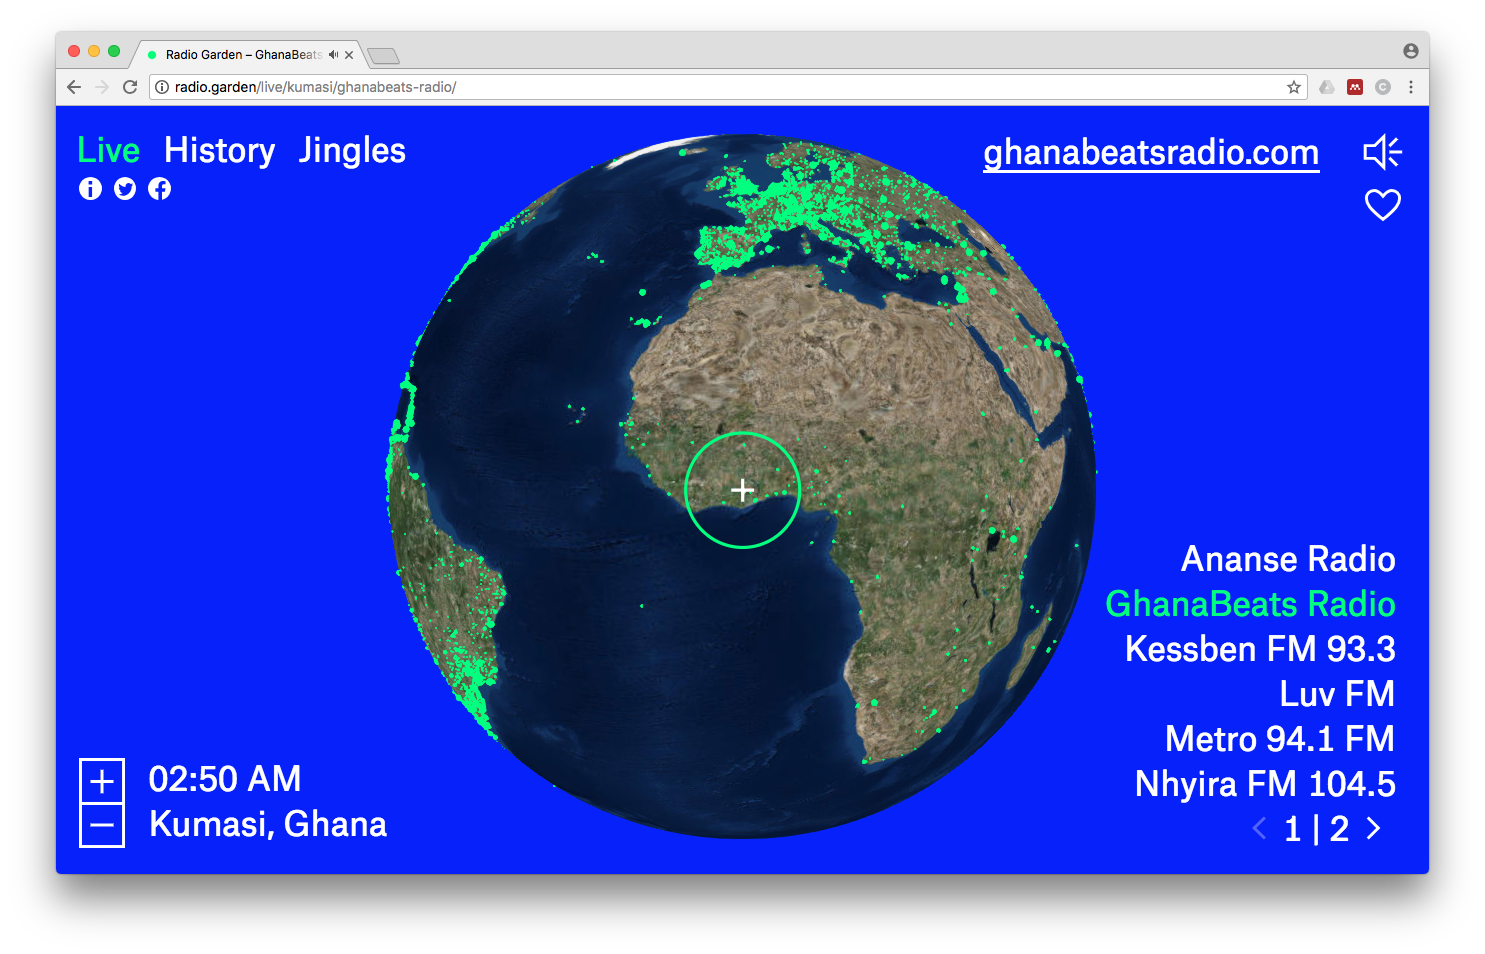
\includegraphics[width=1\linewidth]{pictures/radio_garden_2018-06-10.png}
    \end{center}
    \legend{Fonte: Screenshot da autora, 8 de junho de 2018}
    
\end{figure}
%\legend{Fonte: \citeonline[p. 24]{araujo2012}}

Posso também acessar uma base de dados extensiva da produção humana em música, cinema e televisão construída a partir do trabalho de pessoas em todo o planeta, reunida em grandes portais como o Youtube, onde segundo estatísticas atuais são depositadas 300 horas de conteúdo a cada minuto, mas, como bem apontou a compositora Pauline Oliveros em ``Software for people", ``As mídias e a maior mobilidade obviamente acomodam mais informação, mas não necessariamente mais sabedoria"\cite[179]{Oliveros2012}. 

Os teóricos da sociedade da informação professavam que a internet teria um papel demiúrgico, que ``libertaria a humanidade sem qualquer necessidade de luta de classes" \cite[275]{Barbrook2009}, mas sob a neoliberal "ideologia californiana", a internet se transformou na apoteose do mercado (idem, p. 353). Há quem inclusive culpe a mídia eletrônica por exacerbar uma série de de males da sociedade como: "elitismo, pedofilia, terrorismo, deficiência educacional e solidão" (idem, p. 59). 

\todo[inline]{fake news}

Não é difícil de concordar com essa visão. Uma simples tecnologia que permite ao usuário deixar sua opinião nas notícias dos grandes portais é suficiente para nos assombrar com o nível de barbárie latente na sociedade, a cada notícia veiculada na supostamente isenta ``grande mídia". Abre espaço para a voz do Zé Ninguém, como definido por Wilhem Reich \cite{reich1998escute}, aquele ser de mentalidade tacanha, que "está sempre do lado dos perseguidores" (p. 27), que persegue mães solteiras, por serem imorais, ao mesmo tempo que cultua Jesus, que ``é tolerante com a sua própria religião mas com nenhuma outra (p.51)":

\begin{citacao}
como não tem memória para coisas que aconteceram há dez ou vinte anos, você ainda repete os mesmos disparates de dois mil anos atrás. Pior, você se agarra com unhas e dentes a absurdos como "raça", "classe", "nação" e à obrigação de seguir uma religião e reprimir sua desgraça. \cite[101]{reich1998escute} 
\end{citacao}

Apesar disso, nós, que somos artistas, pesquisadores e pessoas que criam, não podemos nos sujeitar passivamente à essa visão apocalíptica de que a internet está nos levando à barbárie, e podemos pensar nos meios tecnológicos como ponto de partida para novas proposições éticas e estéticas. Concordamos com arquiteto e pintor Sérgio Ferro quando afirma: que a expressão humana na arte é ``pegar a necessidade histórica que está no material e trabalhá-la até o fundo", \cite{FerroSergio2002} e que isto é a própria essência da liberdade.

 \todo[inline]{programação como potencia}

A música, dentre as demais formas de arte é muito potente, no sentido de que o som é quase impossível de se bloquear. Ela tem a capacidade de atingir as pessoas circundantes de uma maneira geral e compulsória, a energia sonora é das mais difíceis de se conter em termos coletivos. É possível um indivíduo tampar seus próprios ouvidos, mas é muito difícil tapar os ouvidos alheios, e mesmo tampando os ouvidos, nunca haverá silêncio. Levinson (1999) aponta que o som tem como característica "emanar de todos ambientes", e enquanto a visão nos dá detalhes preciso, ponto-a-ponto do ambiente ao nosso redor, é a audição que ``nos mantém em contato com o mundo vinte e quatro horas por dia" \cite[47]{Levinson2001}. 

\todo[inline]{Acredito que esse poder pode ser uma das razões pela qual a sociedade patriarcal tende a manter as mulheres longe dos instrumentos musicais.}  

Minha relação com a produção musical teve muita relação com esse potencial de agregação que a música traz, primeiro, como dj, organizando festas que eram essenciais para o financiamento do grêmio dos estudantes da FAU, depois, no Urbando, grupo de maracatu que intervinha também em atos estudantis, e sempre foi muito nítido pra mim o potencial de um tambor ou um xequerê como instrumento de organização de massas em atos, como instrumentos para colocar as pessoas em movimento. Não é atoa que os exércitos usam marchas como forma de elevar a moral dos soldados, e que também as igrejas usem música para encantar os fiéis. O discurso verbal pode ser cansativo, o texto pode ser ignorado, enquanto a música é capaz de colocar uma multidão em uníssono. Em uma sociedade como a nossa, esse poder é exercido principalmente pela indústria cultural, que afasta esse sentido político que a música pode ter, convertendo tudo em mercadoria, como aponta Marilena Chauí no seu artigo "Cultura e Democracia": 

\begin{citacao}

Como cultura de massa, as obras de pensamento e de arte tendem: de expressivas, tornarem-se reprodutivas e repetitivas; de trabalho da criação, tornarem-se eventos para consumo; de experimentação do novo, tornarem-se consagração do consagrado pela moda e pelo consumo; de duradouras, tornarem-se parte do mercado da moda, passageiro, efêmero, sem passado e sem futuro; de formas de conhecimento que desvendam a realidade e instituem relações com o verdadeiro, tornarem-se dissimulação, ilusão falsificadora, publicidade e propaganda. mais do que isso. A chamada cultura de massa se apropria das obras culturais para consumi-las, devorá-las, destruí-las, nulificá-las em simulacros. Justamente porque o espetáculo se torna simulacro e o simulacro se põe como entretenimento, os meios de comunicação de massa transformam tudo em entretenimento (guerras, genocídios, greves, festas, cerimônias religiosas, tragédias, políticas, catástrofes naturais e das cidades, obras de arte, obras de pensamento). É isto o mercado cultural. \cite[61]{MarilenaChaui2008}
\end{citacao}

Uma cultura democrática, seria aquela, segundo ela, onde as pessoas tenham acesso aos meios de produção cultural, e não somente aos produtos de seu mercado. Tendo uma formação em arquitetura e design, e sendo assim de certo modo estranha ao contexto e aos códigos da música tradicional, foi fácil notar o alto grau de fechamento da cena musical, especialmente para mulheres, como aponta Pauline Oliveros no texto ``And don't call them Lady Composers" \cite[48]{Oliveros2012}. Uma das coisas que colabora com esse hermetismo é a dificuldade de acesso aos instrumentos musicais, que podem ser muito caros, pesados ou de difícil manipulação. 

\todo[inline]{Parti minha pesquisa então dessa questão do acesso, uma vez que sendo mulher, pequena e trabalhadora, é uma questão fundamental na minha prática artística cotidiana.}


O acesso aos meios de produção certamente é uma das barreiras que afasta as pessoas de uma vivência musical cotidiana. Instrumentos musicais, equipamentos de áudio em geral e controladores, podem ser muito caros, complexos e de difícil manipulação\cite{Fiebrink2007} . "Ubiquitous music research is not just yet
another approach to musical interaction. It is a new way to foster music making in contexts
that were previously not accessible to artistic endeavors." \cite{Keller2018}

A digitalização das tecnologias de produção musical, no entanto, tornou acessível aos usuários de computadores pessoais, tecnologias que só eram disponíveis para grandes estúdios musicais. A partir dos anos 80, isso causou um crescimento exponencial do engajamento da juventude com meios de produção musical digitais, como aponta Georgina Born \cite[143]{Born2015}, mas também causa a uma "tecnofilia fetichista" em relação a equipamentos e tecnologias (idem, p. 145).

Como aponta Baudrillard em ``O sistema de objetos", ``os consumidores não têm acesso à igualdade diante do objeto depois da Revolução Industrial" \cite[162]{Baudrillard2012}. Podemos dizer que a revolução digital, tem permitido concentrar uma série de funcionalidades em gadgets como celulares ou laptops, cada vez menores e mais complexos, que exercem cada vez mais uma dominação dos sentidos individuais das pessoas – que ficam dependentes e absortas em complexas tramas de dados e dramas. O gadget para Baudrillard é um objeto que faz parte de um universo de delírio funcional, um tecnicismo excêntrico e formalismo gratuito, objetos tomados totalmente pelo imaginário, ou obsessões pura e simples, aberrações funcionais. (idem p.121). 

Meu projeto parte de um desejo de libertação dessa dependência de toda uma uma parafernália tecnológica, concentrando esforços em desenvolver protótipos experimentais para produção musical em tecnologias para a rede. Soluções deste tipo podem ser mais acessíveis, já que um instrumento musical online poderia ser acessado por qualquer dispositivo que tenha acesso à internet -- como computadores ou smartphones -- gadgets que ganharam muito poder de processamento, nos quais já estamos absortos. Além disso, tinha um desejo sobretudo de investigar novas formas de interface, por considerar que muitas das interfaces existentes, que são em maioria baseadas nas de equipamentos eletrônicos \cite{Stolfi2016}, também exigem a necessidade de saberes bastante específicos em tecnologias musicais, além de imporem certos parâmetros da música tradicional, como notas, timbres e tempos. 

Com o desenvolvimento da pesquisa, e o meu contínuo envolvimento com práticas musicais como a da improvisação livre, ``uma pragmática musical aberta à variação infinita em que os sistemas e as linguagens deixam de impor suas gramáticas abstratas e se renderem a um fazer fecundo" \cite[2]{Costa2016} esse desejo de construção de instrumentos genéricos foi se direcionando para a construção de instrumentos específicos para suprir necessidades pessoais musicais -- como é o caso do projeto Banda Aberta e o Playsound, projetos que descreverei mais a frente nesta tese -- sempre buscando portabilidade e facilidade de uso.


\subsection{interfaces não gesturais}

Na música tradicional, o gesto -- do performer ou do intérprete -- é tradicionalmente o gerador do som. O domínio do ato de tocar, principalmente instrumentos tradicionais, envolve um domínio de uma linguagem corporal que gera o som desejado de acordo com o desejo do musicista. Na música instrumental e vocal, sempre há um gesto físico que gera o som, o que não acontece necessariamente na música eletrônica \cite[85]{Smalley1996}. Isto é uma preocupação de quem desenvolve aplicativos para música interativa, como aponta Schnell (2013). 


\begin{citacao}
Two principal concerns constitute the design of interactive audio applications and musical in- struments of virtually any kind. One deals with creating real-time interactive sound processes and the other with the way these sound processes are influenced by the bodily movements and gestures of their players. In this sense, the essence of designing interactive audio applications lies in the creation of meaningful relationships between movement – or gestures – and sound. \cite{Schnell2013}
\end{citacao}
Essa questão já é discutida no âmbito das laptop orchestras, como aponta Trueman (2007):
\begin{citacao}
For the laptop performer, this seems to pose a
deep problem. If we look like we are simply doing e- mail while generating sounds that provoke the motor-mimetic response of, say, striking an enormous hammer, what will the ‘listener’ make of it all? What kind of vicarious performance could this possibly inspire?What would the ‘air-laptop’ dance look like? 
But perhaps this is an opportunity instead of a problem, a challenge for which the laptop orchestra is a musically and socially charged gymnasium. On the one hand, we can go at it head-on and endeavour to create challenging instruments that generate sounds which somehow seem tangibly (even acoustically) related to the physicality they demand.





\cite[6]{Trueman2007}
\end{citacao}

\subsection{agência}


A noção de virtuosidade, para Smalley (1996) é baseada na identificação de um controle consumado na articulação de morfologias sonoras. No seu modelo do espectro de sons, Smalley considera como sons musicais, aqueles gerados com intenção pelos homens, mesmo sons naturais, podem ser convertidos em música desde que sejam resultado de uma agência humana. O campo da música eletroacústica foi responsável por inserir na música uma ampla gama de sons sintetizados e da natureza que não necessariamente podem nem ter tido uma existência material. Muitos trabalhos acusmáticos, inclusive, não possuem nenhuma fonte sonora gestual visível em tempo real \cite[95, 101]{Smalley1996}.



\todo[inline]{Para estruturar essa pesquisa em uma tese de doutorado, partirei de uma conceituação teórica a respeito de alguns temas que norteiam essa pesquisa: 
o princípio da antropofagia, que envolve procedimentos práticos e teóricos da nossa metodologia; 
a idéia de interdisciplinaridade como prática, e relações estabelecidas entre design, música e tecnologia; 
a idéia de cultura livre, defendida por uma série de ativistas da cultura digital; 
a estética do brutalismo digital verbivocovisual e suas referências históricas; 
a noção de música prática e experimental como espaço de liberdade.
Em seguida, vou reunir alguns recursos utilizados durante esta pesquisa, de modo a fornecer uma base de conhecimentos para quem se interesse por práticas semelhantes. Tratarei de recursos como servidores de internet, ferramentas e linguagens úteis até e recursos para produção de performance e apresentações tentado buscar um set-list mínimo de equipamentos e cabos. 
O capítulo seguinte, tratará do processo de pesquisa em si, partindo de primeiras experiências de pesquisa em redes e em interfaces para produção e difusão musical, como a música me levou à internet e como a internet me levou à música, através de práticas junto a coletivos, grupos de discussão e práticas artísticas em grupo, até os experimentos desenvolvidos junto ao grupo de pesquisa NuSom, na Universidade de São Paulo, como o projeto Banda Aberta, o Spectrogram player e outras experiências em música interativa que estou desenvolvendo. 
Por fim, apresentarei nas considerações finais, algumas questões éticas e estéticas levantadas  ao longo da pesquisa, conclusões e resultados dos experimentos aqui desenvolvidos, bem como limitações e potencialidades para desenvolvimentos futuros.
}


\subsection{Cultura Livre}

Procuramos defender uma idéia de cultura livre, que permeia uma série de práticas, desde a escolha das linguagens, do repertório e dos projetos, até a publicação de código aberto e conteúdo em licenças livres. A própria adoção de práticas de improvisação livre tem relação com essa idéia. A digitalização da arte leva à possibilidade de livre reprodução, e amplia sua sua exponibilidade, como já apontava Benjamin (1987). A própria web foi construída com base em idéia de livre circulação da informação, na adoção de uma estrutura não hierárquica e de linguagens livres de marcação (Berners-lee, 1989).
A cultura livre é defendida por uma comunidade de pensadores, programadores e artistas, como Lawrence Lessig (2004), e a iniciativa Creative Commons, Richard Stallman e a comunidade do software livre, e mesmo Alexandra Elbakyan com o Scihub que desafia constantemente a propriedade da informação, (Barok et al, 2015) entre vários outros que têm constantemente militado por diversas práticas culturais libertárias.

\begin{citacao}
Durante a explosão ponto com do final dos anos 1990, Richard Stallman – um cientista da computação do MIT e guru da Fundação do Software Livre (Free Software Foundation) – resistiu fi rmemente à pressa em comercializar a Internet. Fiel à visão de Licklider, ele defendeu a ética hacker de esforço coletivo e investigação aberta. Da perspectiva dos laboratórios de pesquisa universitários, os pro gramas de computador proprietários possuíam um defeito de fábrica intrínseco: restrições de propriedade intelectual. Dentro da economia da dádiva acadêmica, programadores eram encorajados a compartilhar, apropriar e melhorar o trabalho de todos. Em oposição, a Microsoft e outras empresas comerciais guardavam enciumadas os segredos de seus códigos-fonte. Os usuários de computador foram impedidos de tornarem-se, além de consumidores, produ- tores de programas.\cite[367]{Barbrook2009}
\end{citacao}


\begin{citacao}
Na arquitetura aberta da
Internet, as restrições da propriedade intelectual tornavam-se um anacronismo. Embora produtores ainda pudessem impedir que seu trabalho fosse apropriado por outros, todos deveriam ser autorizados a copiar e alterar informações para seus próprios propósitos. Em meados dos anos 1990, Stallman lançou uma campanha para as leis de propriedade intelectual dos Estados Unidos serem reformadas de acordo com o método de trabalho ao estilo universitário: “copyleft” \cite[368]{Barbrook2009}
\end{citacao}



\subsection{Brutalismo Digital}
Neste subtema, procurarei falar de referências estéticas, e especialmente da influência da arquitetura moderna e do brutalismo de Vilanova Artigas e da precariedade radical de Lina Bo Bardi, dos concretistas russos como El Lissitsky e Rodchenko e brasileiros como Sacilotto, Athos Bulcão e Lygia Pape, Erthos Albino de Souza, Augusto de Campos, Haroldo de Campos e Décio Pignatari. Trabalhar a partir de  referências do passado pode trazer certas questões ideológicas, como aponta Plaza (idem, p. 6):
Operar sobre o passado encerra um problema de valor. Não é escolher um dado do passado, uma referência passada; é uma referência a uma situação passada de forma que seja capaz de resolver um problema presente e tenha afinidade com suas necessidades precisas e concretas, de modo a projetar o presente sobre o futuro. Toda época distingue entre formas conservadoras e mais inovadoras. As inovadoras são as que se projetam para o futuro através do caráter inacabado que aponta para um possível leitor, o que é também uma forma de ``perceber na cultura de hoje os traços reais e inconfundíveis do amanhã''. Operar sobre o passado, além de um problema de valor, constitui-se também numa operação ideológica através da qual podemos confirmar a produção do presente ou encobrir essa realidade. Se, no primeiro caso se favorece um encontro dialético com o passado para preparar o futuro, no segundo, trata-se de distanciar esse futuro indefinidamente. No primeiro caso, os valores da história constituem-se num modelo para a ação, já no segundo, trata-se de um fantasma a ser evocado como nostalgia, moda ou revival.
Aqui, não queremos trazer essas referências como inspiração ou nostalgia, mas como apontamentos para pensar possibilidades estéticas. Como os princípios de racionalidade,  e sobretudo uma postura anti-decorativa, anti-ornamental e de procurar um mínimo de elementos necessários. 

\subsection{Trans-disciplinaridade}
No artigo "Logics of interdisciplinarity", Barry, Born e Weszalnys apontam o campo interdisciplinar da Arte-ciência, como um campo emergente, onde "a prática corre na frente da teoria" (BARRY, A.; BORN, G.; WESZKALNYS, G, 2008, p. 38), que pode ter como um dos objetivos "desafiar e transformar formas existentes de pensar sobre a natureza da arte e da ciência, bem como as relações entre artistas e cientistas e seus objetos e públicos" , segundo eles, invenção e originalidade na arte-ciência se sustentam melhor nas práticas onde os artistas conseguem fazer uso de laboratórios, oficinas e computadores (idem, p. 39). Isto é reforçado se observarmos os trabalhos de alguns pioneiros da arte digital, como Erthos Albino de Souza, Waldemar Cordeiro, Nam Jum Paik e Júlio Plaza. 
Plaza aponta que intermídia e multimídia são "categorias interdisciplinares  que colocam em questão as formas de produção-criação individual"  (Plaza, 2013 p. 66) e que as formas eletrônicas tem um caráter abrangente que dialoga "intersensorialmente" com vários códigos da informação, "uma hibridização de meios, códigos e linguagens que justapõem e se combinam" (idem, p. 13)

\subsection{Antropofagia}

    % Write epigraphs
    \begin{flushright}
        \textit{``A síntese
O equilíbrio
O acabamento de carrosserie
A invenção
A surpresa
Uma nova perspectiva
Uma nova escala
Qualquer esforço natural nesse sentido será bom.''} \\
Oswald de Andrade – Manifesto Pau Brasil    \end{flushright}

``A alegria é a prova dos nove'', aponta Oswald no Manifesto Antropófago. Desde meus primeiros envolvimentos com música e performance no Coro de Carcarás, por volta de 2005, a influência da antropofagia Oswaldiana foi bastante significativa. Neste capítulo procurarei tratar especificamente desta influência, bem como da de artistas que tomaram esse princípio para suas práticas, como Lygia Clark e Hélio Oiticica, neste que tem um certo aspecto de devoração do outro e um sentido de busca de alegria e liberdade, relacionando também com práticas correntes junto a redes como a do tecnoxamanismo, que trouxeram novas perspectivas neste sentido.

\subsection{Música Prática}

\begin{citacao}


The hardest thing for a digital musician to decide is not what skills should be acquired but what not to learn. Given that the skill set draws upon so many different and well- established disciplines, it is always possible to go further into any one of them in order to specialise in a particular area. A theme that emerges, there- fore, is the sheer number and variety of employment situations or careers. Here is a quick list of just some of them: programmer, music and effects for games, music and effects for cinema (location sound, ADR, Foley, sound effects, re-recording engineer, composer, session engineer, etc.), music and effects for industrial video, audio- loops designer, audio- effects designer, mobilephone ringtone designer, radio producer, studio engineer, record producer, mastering engineer, music- related retail sales, music software support, jingle writing, music- events producer, live- sound engineer, band member, session musician, arts administrator, self- promoted musician, Internet- based microsales, record- label manager, talent scout, A\&R (artist and repertoire) representative, acoustic designer, arts/sound museum\/events coordinator, events\/festivals technical support, PA system con- sulting and installation, DSP inventor, instrument inventor, writer for electronic music magazines, sound for web (commercial record sales samples, sound design for sites, interactive sound), bulk media reproduction, teaching, music therapy, new- age market (relaxation tapes, mind manipulation, etc.), Muzak, corporate sonic environments, multimedia development, busking, lawyer, music librarian, artist.\cite[191]{Hugill2012}
\end{citacao}


gravação, edição e sequenciamento
processamento de sinais (incluindo plugins)
samplers
instrumentos virtuais (vst)
sintetizadores
performance ao vivo
notação
composição
análise e representação
modulares ou construíveis

\begin{citacao}
Music production relies on software. To specify precisely which music software packages might be useful to the musician is futile, because the software market changes so rapidly. However, it is possible to identify generic types of music soft- ware, as follows:
• sound recording, editing and sequencing software • processing applications (including plug- ins) • software samplers • virtual instruments • synthesis software • live- performance software • notation software • composition software • analysis or representation software • modular or build- it- yourself software.\cite[195]{Hugill2012}
Additions
\end{citacao}


The digital musician will need to be aware that such software can try to steer musical content in a particular direction, even towards a specifi c genre or style. Sometimes music production is a matter of fi nding ways to achieve some- thing original in spite of the software design. \cite[195]{Hugill2012}


\begin{citacao}
A nosso ver, se devemos operar \emph{em} e \emph{para} um mundo construído na medida humana, essa medida será individuada não adaptando o homem a essas condições de fato mas \emph{a partir dessas condições de fato}. O universo das comunicações de massa é -- reconheçamo-lo ou não -- o nosso universo; e se quisermos falar de valores, as condiçnoes objetivas das comunicações são aquelas fornecidas pela existência dos jornais, do rádio, da televisão, da música reproduzida e reproduzível, das novas formas de comunicação visiva e auditiva. Ninguém foge a essas condições, nem mesmo o virtuoso, que, indignado com a natureza inumana desse universo da informação, transmite o próprio protesto através dos canais de comunicação em massa, pelas colunas do grande diário, ou nas páginas do volume em \emph{paperback}, impresso em linotipo e difundido nos quiosques das estações.\cite[13]{Eco1970}


\end{citacao}

estamos em plena indústria cultural, e um operador de cultura, deve segundo Eco
\begin{citacao}
Colocar se em relação dialética, ativa e consicente com os condicionamentos da indústria cultural tornou-se para o operador de cultura o único caminho para cumprir sua função. \cite[14]{Eco1970}
\end{citacao}

\begin{citacao}
Em 1983, Ithiel de Sola Pool – um antigo funcionário da Cenis e membro da Comissão Bell – codifi cou sua apropriação neoliberal do mcluhanismo na sua obra principal, Technologies of freedom (Tecnologias da liberdade). Ao invés de construir a ágora eletrônica, a convergência da mídia, das telecomunicações e da computação criava o mercado eletrônico. De programas de computadores a novelas, todas as formas de informação seriam logo negociadas como mercadorias pela Internet. Pela primeira vez, todos poderiam ser um empreendedor de mídia. \cite[348]{Barbrook2009}
\end{citacao}

\begin{citacao}

Para o seu colega da Wired, Howard Rheingold, a Internet também
foi a curandeira da alienação social. Em sua atualização da Nova,
Esquerda mcluhanista do início dos anos 1990, BBSs, MUDsNT2
serviços de bate-papo instantâneos e servidores de lista de e-mail representavam os princípios da ágora eletrônica postos em prática: as “comunidades virtuais”. Fundada sobre o compartilhamento de informação e conhecimento, a Internet era uma das “ferramentas para pensar” que liberariam a humanidade da sociedade fabril fordista. \cite[350]{Barbrook2009}
\end{citacao}

\begin{citacao}
Como herdeiros de Hilferding e Stalin, esquerdistas tradicionais acentuaram que as indústrias culturais não poderiam escapar aos processos de monopolização e centralização que moldavam todos os setores da economia capitalista.68
Com mais sensacionalismo,
outros acadêmicos apocalípticos culparam a mídia eletrônica e os computadores por exacerbarem uma larga variedade de males sociais: elitismo, pedofi lia,
terrorismo, defi ciência educacional e solidão.69 Gilles Deleuze – um fi lósofo veterano da Nova Esquerda
– advertiu que as novas tecnologias da informação forneciam a infra- estrutura de monitoramento e vigilância da autoritária “sociedade de controle” emergente. Ao invés de emancipar as massas, o advento da Internet ameaçava reforçar o poder de seus opressores. “Comparado com as formas que se aproximam de contínuo controle em lugares abertos, nós veremos talvez o mais severo dos confi namentos como parte de um passado maravilhosamente feliz. A busca por ‘universais de comunicação’ pode nos fazer tremer”.\cite[359]{Barbrook2009}
\end{citacao}


    \newpage

     \emph{}

    \section*[Some encoding tests]{Some encoding tests}

    % Why latex is letting my text goes out of the screen?
    % https://tex.stackexchange.com/questions/386762/why-latex-is-letting-my-text-goes-out-of-the-screen
    \sloppy
    \textbf{textbf:  }
    \fussy

\end{otherlanguage*}




A Tabela~\ref{tab:a_table_formatacao_de_texto} mostra mais informações do template BU.

% What does [t] and [ht] mean?
% https://tex.stackexchange.com/questions/8652/what-does-t-and-ht-mean
%
% How can I get rid of the LaTeX warning: Float too large for page?
% https://tex.stackexchange.com/questions/36252/how-can-i-get-rid-of-the-latex-warning-float-too-large-for-page
%
% "warning: Text page X contains only floats" How to suppress this warning?
% https://tex.stackexchange.com/questions/223149/warning-text-page-x-contains-only-floats-how-to-suppress-this-warning
%
% Make a table span multiple pages
% https://tex.stackexchange.com/questions/26462/make-a-table-span-multiple-pages
%
% How to make the longtable to work with centering & caption on memoir class?
% https://tex.stackexchange.com/questions/386541/how-to-make-the-longtable-to-work-with-centering-caption-on-memoir-class
%
% How to fix this Package array Error: Only one column-spec allowed?
% https://tex.stackexchange.com/questions/367069/how-to-fix-this-package-array-error-only-one-column-spec-allowed
%
% How to auto adjust my last table column width, and why is there Underfull \vbox badness on this table?
% https://tex.stackexchange.com/questions/387238/how-to-auto-adjust-my-last-table-column-width-and-why-is-there-underfull-vbox/387251
\setlength\extrarowheight{2pt}
\begin{tabularx}{\linewidth}{>{\RaggedRight}p{3cm}|>{\arraybackslash}X}

\caption{Formatação do texto \protect }
\label{tab:a_table_formatacao_de_texto} \\
\hline
\endfirsthead

% How to set font size of footnotes correctly in memoir?
% https://tex.stackexchange.com/questions/213927/how-to-set-font-size-of-footnotes-correctly-in-memoir
\multicolumn{2}{p{\dimexpr\textwidth-2\tabcolsep\relax}}{\ufsccaptionsize\tablename~\thetable:
Formatação do texto (continuação) \protect } \\
\hline
\endhead

% Set multicolumn width to default table width
% https://tex.stackexchange.com/questions/99326/set-multicolumn-width-to-default-table-width
\hline
\multicolumn{2}{p{\dimexpr\textwidth-2\tabcolsep\relax}}{\footnotesize continua na próxima página\protect }
\endfoot

\hline
\endlastfoot

    Cor                          & Branco -                                                 \\ \hline
    Formato do papel             & A5                                                               \\ \hline
    Gramatura                    & 75                                                               \\ \hline
    Impressão                    & Frente e verso                                                   \\ \hline
    Margens                      & Espelhadas: superior 2, Inferior: 1,5, Externa 1,5 e Externa: 2. \\ \hline
    Cabeçalho                    & 0,7                                                              \\ \hline
    Rodapé                       & 0,7                                                              \\ \hline
    Paginação                    & Externa                                                          \\ \hline
    Alinhamento vertical         & Superior                                                         \\ \hline
    Alinhamento do texto         & Justificado                                                      \\ \hline
    Fonte sugerida               & Times New Roman                                                  \\ \hline
    Tamanho da fonte             & 10,5 para o texto incluindo os títulos das seções e subseções.
                                   As citações com mais de três linhas as legendas das ilustrações
                                   e tabelas, fonte 9,5.                                            \\ \hline
    Espaçamento entre linhas     & Um (1) simples                                                   \\ \hline
    Espaçamento entre parágrafos & Anterior 0,0; Posterior 0,0                                      \\ \hline
    Numeração da seção           & As seções  primárias devem  começar  sempre em páginas ímpares.
                                   Deixar um espaço (simples) entre o título da seção e o texto e
                                   entre o texto e o título da subseção.                            \\ \hline

\end{tabularx}











